% -*- TeX-master: "main"; fill-column: 72 -*-

\section{Examples}
\label{examples}

\subsection{Graphical and typographical conventions}

This proposal mainly covers logical models but it can also handle standard Petri nets. We provide below one example for each.
%the examples are labeled with a token indicating the corresponding formalism : \ALL all formalisms, \PN Petri nets, \LRG logical regulatory networks or \SYM symbolic relationships.

\subsection*{Simple Logical Regulatory Graph} % (fold)
\label{sub:lrg}
%\LRG 
The following example shows a simple LRG with 3 regulators A, B and C, where A can take three values ($A=\{0,1,2\}$), and B,C are Boolean. Moreover, A positively regulates B, which positively regulates C, whith positively regulates A. In turn A activates itself at level 1 but inhibits itself at a higher level (2) (see figure below).

The logical functions are the following:

\begin{center}

$\begin{array}{lr}
      $B := 1$ & \mbox{if $A => 1$} \\
      $C := 1$ & \mbox{if $B => 1$} \\
     \end{array}
$

$
A :=\left\{ \begin{array}{cl}
      2 & \mbox{if $(1 <= A < 2) or (C >= 1)$} \\
      1 & \mbox{if $A < 1 and C >= 1$} \\
      0 & \mbox{otherwise}  \\
     \end{array}
\right.
$
\end{center}

\begin{figure}
\centering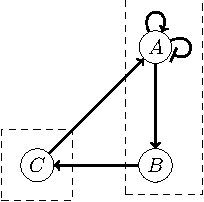
\includegraphics{figs/LRG.pdf}
\end{figure}


\lstinputlisting[caption=Logical Regulatory Graph example,label=ex_LRG]{Examples/example.sbml}

% subsection lrg (end)
\bigskip
\subsection*{Simple Petri net} % (fold)
\label{sub:ex_pn}
%\PN 
The following example shows a simple, standard Petri net, with 4 places A, B, C and D and one transition $t1$ as depicted in the figure below.
\begin{figure}
\centering
\includegraphics{figs/PN.pdf}
\end{figure}

\lstinputlisting[caption=Petri net example,label=ex_pn_listing]{Examples/examplePetri.sbml}

% subsection ex_pn (end)

% section use-cases and examples (end)
